\documentclass[12pt,a4paper]{report}
\usepackage[utf8]{inputenc}
\usepackage[francais]{babel}
\usepackage[T1]{fontenc}
%\usepackage{fontspec}
\usepackage{amsmath}
\usepackage{amsfonts}
\usepackage{amssymb}
\usepackage{amsthm}
\usepackage{makeidx}
\usepackage{gensymb}
\usepackage{graphicx}
\usepackage{lmodern}
\usepackage{hyperref}
\usepackage{cancel}
\usepackage{siunitx}
\usepackage{blindtext}
\usepackage{xcolor}
\usepackage{cite}
\usepackage[explicit]{titlesec}
%\usepackage[numbers]{natbib}
%\usepackage[round]{natbib}   % omit 'round' option if you prefer square brackets
%\usepackage[square,sort,comma,super,authoryear]{natbib}
\everymath{\displaystyle}
\usepackage[final]{pdfpages}
%\usepackage{kpfonts}
%\usepackage{fourier}
\usepackage{fancyhdr}
\pagestyle{fancy}
%\fancyhf{}
\fancyhead[R]{\footnotesize\rmfamily\nouppercase\leftmark}
\fancyhead[L]{\footnotesize\rmfamily\nouppercase\rightmark}

%----------------------------arabic setting--------------------------------------------
\iffalse
   %\setmainfont[Ligatures=TeX]{Times New Roman}
   \newfontfamily\arabicfont
      [Script=Arabic,     % to get correct arabic shaping
        Scale=1.2]          % make the arabic font bigger, a matter of taste
        {Arial}     % whatever Arabic font you like

   \newcommand{\textarabic}[1]     % Arabic inside LTR
       {\bgroup\textdir TRT\arabicfont #1\egroup}
   \newcommand{\n}         [1]     % for digits inside Arabic text
       {\bgroup\textdir TLT #1\egroup}
   \newcommand{\afootnote} [1]     % Arabic footnotes
       {\footnote{\textarabic{#1}}}
   \newenvironment{Arabic}     % Arabic paragraph        {\textdir TRT\pardir TRT\arabicfont}{}
   {\textdir TRT\pardir TRT\arabicfont}{}
\fi
%--------------------------------------------------------------------------------


%_______________________dont allow breaking math mode_______________________________________________
\relpenalty=10000
\binoppenalty=10000
%________________________________________________________________________________________









\theoremstyle{plain}
\newtheorem{theo}{\textit{Théorème}}[chapter]
\newtheorem{pro}{\textit{Proposition}}[chapter]
\newtheorem{corl}{\textit{Corollaire}}[chapter]
\newtheorem{cons}{\textit{Conséquence}}[chapter]
\newtheorem{lem}{\textit{Lemme}}[chapter]
\newtheorem{exo}{Exercice}

\theoremstyle{definition}
 \newtheorem{defn}[theo]{\textit{Définition}}
 \theoremstyle{remark}
\newtheorem{rem}{\textit{Remarque}}[chapter]
\newtheorem*{exm}{\textit{Exemple}}
\newtheorem*{nott}{\textit{Notation}}






















%------------------------------raccourcis pour les notations---------------------------
\newcommand{\Cn}{\ensuremath{\mathbb{C}^n}}
\newcommand{\Cnn}{\ensuremath{\mathbb{C}^{n+n'}}}
\newcommand{\Cnm}{\ensuremath{\mathbb{C}^{n+m}}}
\newcommand{\Cnmm}{\ensuremath{\mathbb{C}^{n+2m}}}
\newcommand{\C}{\ensuremath{\mathbb{C}}}
\newcommand{\Z}{\ensuremath{\mathbb{Z}}}
\newcommand{\N}{\ensuremath{\mathbb{N}}}
\newcommand{\Np}{\ensuremath{\mathbb{N}^p}}
\newcommand{\Nnn}{\ensuremath{\mathbb{N}^{n'}}}
\newcommand{\Nq}{\ensuremath{\mathbb{N}^q}}
\newcommand{\Cx}{\ensuremath{\mathbb{C} \{x\}}}
\newcommand{\Cfx}{\ensuremath{\mathbb{C} [[x]] }}
\newcommand{\Nn}{\ensuremath{\mathbb{N}^n}}
\newcommand{\Zn}{\ensuremath{\mathbb{Z}^n}}
\newcommand{\Zp}{\ensuremath{\mathbb{Z}^p}}
\newcommand{\M}{\ensuremath{\mathbb{R}}}
\newcommand{\Mpp}{\ensuremath{\mathbb{R}^p}}
\newcommand{\Mq}{\ensuremath{\mathbb{R}^q}}
\newcommand{\Mr}{\ensuremath{\mathbb{R}^r}}
\newcommand{\Mn}{\ensuremath{\mathbb{R}^n}}
\newcommand{\Mpq}{\ensuremath{\mathbb{R}^p\times \mathbb{R}^q}}
\newcommand{\ZpNq}{\ensuremath{\mathbb{Z}^p\times \mathbb{N}^q}}
\newcommand{\Me}{\ensuremath{\mathbb{R}^*}}
\newcommand{\Mp}{\ensuremath{{\mathbb{R}}_+}}
\newcommand{\Mep}{\ensuremath{{\mathbb{R}}_+^*}}
\newcommand{\xn}{\ensuremath{(x_1,\cdots ,x_n)}}
\newcommand{\xp}{\ensuremath{(x_1,\cdots ,x_p)}}
\newcommand{\xr}{\ensuremath{(x_1,\cdots ,x_r)}}
\newcommand{\yq}{\ensuremath{(y_1,\cdots ,y_q)}}
\newcommand{\alf}{\ensuremath{(\alpha_1,\cdots ,\alpha_n)}}
\newcommand{\fr}{\ensuremath{\varphi_R}}
\newcommand{\frx}{\ensuremath{\varphi_R(\xi .x)}}
\newcommand{\Brx}{\ensuremath{B_R(\xi)}}
\newcommand{\Br}{\ensuremath{B_R}}



%-------------------citations pour les chapitres---------------------------------------
\makeatletter
%\renewcommand{\@chapapp}{}% Not necessary...
\newenvironment{chapquote}[2][2em]
  {\setlength{\@tempdima}{#1}%
   \def\chapquote@author{#2}%
   \parshape 1 \@tempdima \dimexpr\textwidth-2\@tempdima\relax%
   \itshape}
  {\par\normalfont\hfill--\ \chapquote@author\hspace*{\@tempdima}\par\bigskip}
\makeatother
%---------------------------------------------------------------------------------------

\newlength\chapnumb
\setlength\chapnumb{4cm}

\titleformat{\chapter}[block]
{\normalfont\sffamily}{}{0pt}
{\parbox[b]{\chapnumb}{%
   \fontsize{120}{110}\selectfont\thechapter}%
  \parbox[b]{\dimexpr\textwidth-\chapnumb\relax}{%
    \raggedleft%
    \hfill{\LARGE#1}\\
    \rule{\dimexpr\textwidth-\chapnumb\relax}{0.4pt}}}
\titleformat{name=\chapter,numberless}[block]
{\normalfont\sffamily}{}{0pt}
{\parbox[b]{\chapnumb}{%
   \mbox{}}%
  \parbox[b]{\dimexpr\textwidth-\chapnumb\relax}{%
    \raggedleft%
    \hfill{\LARGE#1}\\
    \rule{\dimexpr\textwidth-\chapnumb\relax}{0.4pt}}}






%______________________l'espace entre lignes _______________________________________________________
%\setlength{\parindent}{2em}
%\setlength{\parskip}{1em}
%\renewcommand{\baselinestretch}{1.3}
%--------------------------------page de garde---------------------------------------
\author{Abdelhakim Dahmani}
\title{Le Problème de Goursat dans un espace de Carleman }
\date{\today}


%-------------------------------------begin-document-----------------------------------
\begin{document}

\includepdf[pages=-]{pgarde/pgarde.pdf}
\pagenumbering{roman}
\setcounter{chapter}{-1}
%\maketitle
%----------------------------dedicace---------------------------------------------
%\addcontentsline{toc}{chapter}{Dedicace}
\chapter*{Dedicace}
%\vspace*{\stretch{1}}
%\begin{flushright}
 \begin{center}
Je dédie ce travail \\ 
à mes parents.\\
à mes soeurs, et à mon frère.\\
à la mémoire de mes grand-pères, et de ma grande-mère.

 \end{center}
 
 
 

%\end{flushright}
%\vspace*{\stretch{2}}
 
 %\begin{array}
  
  %\hfill 
    
  %\end{array} 
  \vfill \hfill
  \begin{tabular}{c}
   Abdelhakim   Dahmani \\
   Ghardaia   2018
  \end{tabular}
%\thispagestyle{plain}

%-----------------------------------------------------------------------------------

\include{remerciment}
%


%----------------------------résume en français et anglais ----------------------------

\addcontentsline{toc}{chapter}{Résumé}
\chapter*{Résumé,Abstract,molakhas}
\begin{center}
\textbf{\textit{Résumé}}
\end{center}

Dans ce mémoire on s'intéresse à un résultat d'éxistence et d'unicité pour le problème de Goursat non-linéaire dans un espace de Carleman, on transforme le problème integro-différentiel à un problème de point fixe dans une algèbre de Banach définie par le formalisme de certain série formelle construit à partir une suite logarithmiquement convexe à croissance contrôlé 

\textbf{\textit{Mots clés:}} Problème de Goursat, Point fixe, Algèbre de Banach, série formelle, classe de Carleman.
\begin{center}
\textbf{\textit{Abstract}}
\end{center}
In this thesis one is interested in a result of existence and uniqueness for the non-linear Goursat problem in a Carleman space, one transforms the integrodifferential problem into a problem of a fixed point in a Banach algebra defined by the formalism of certain formal power series constricted  by a logarithmic convex sequence with controlled increasing

\textbf{\textit{Keywords:}} Goursat problem, fixed point,Banach algebra,formal power series,Carleman space

\begin{center}
\textbf{\textit{Résumé!!}}
\end{center}

Dans ce mémoire on s'intéresse à un résultat d'éxistence et d'unicité pour le problème de Goursat non-linéaire dans une classe de Carleman, on transforme le problème integro-différentiel en un problème de point fixe dans une algèbre de Banach définie par le formalisme de certain série formelle construit à partir une suite logarithmiquement convexe à croissance contrôlé 

\textbf{\textit{Mots clés:}} Problème de Goursat, Point fixe, Algèbre de Banach, série formelle, classe de Carleman.



%\thispagestyle{plain}

% pour une page sans en-tête ni pieds de page
%\chapter*{Résumés}
%\addcontentsline{toc}{chapter}{Résumé}%Pour l'ajout dans la table des matières au même rang que chapitre
%\begin{abstract}
%Dans ce mémoire on s'intéresse à un résultat d'éxistence et d'unicité pour le problème de Goursat non-linéaire dans un espace de Carleman, on transforme le problème integro-différentiel en un problème de point fixe dans une algèbre de Banach définie par le formalisme de certain série formelle construit avec une suite logarithmiquement convexe à croissance contrôlé 
%\end{abstract}
%\thispagestyle{plain}
%\thispagestyle{empty}%idem pour la page blanche qui suit
%\selectlanguage{english}% pour un typographie anglaise
%\renewcommand{\abstractname}{Abstract}%pour changer le titre
%\begin{abstract}
%My abstract: vous pouvez notez ici que l'espacement entre le mot abstract et les : n'est pas le même qu'en français, comme le veut la typographie anglaise.
%\end{abstract}
%\thispagestyle{plain}

%\thispagestyle{empty}%
%\selectlanguage{french}% on n'oublie pas de repasser en langue française.
%---------------------------------------------------------------------------------

%\include{résumé}
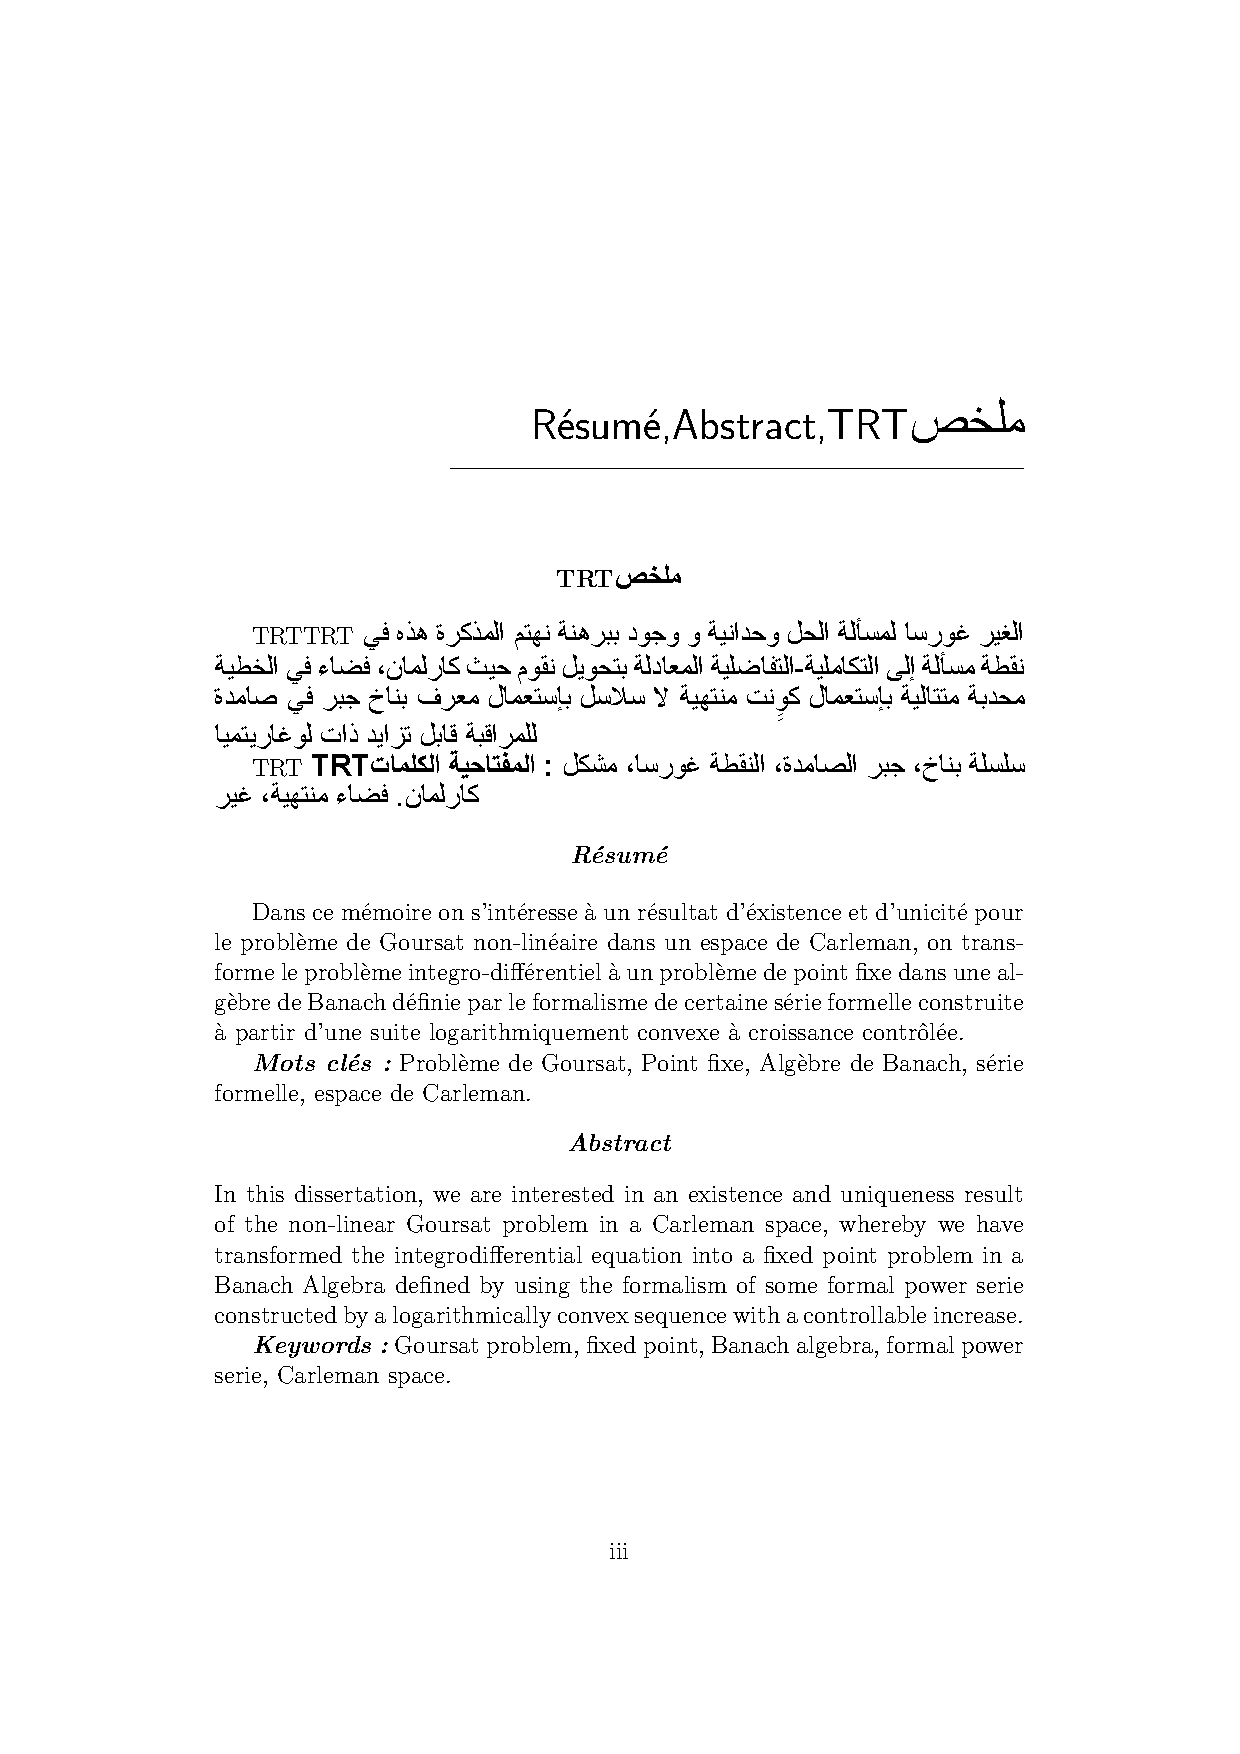
\includepdf[pages=-]{resumesepare/resumesepare.pdf}
 






%\addcontentsline{toc}{chapter}{Table des matières}
\tableofcontents

\addcontentsline{toc}{chapter}{Notation}
\chapter*{Notation}
Soient $\alpha, \beta \in \Zn$, $ x,y \in \Cn \text{ ou }\Mn$ \\
\iffalse
$\ \ \ \  $\\
$\bullet\ \ \ \ \Cx  $:l'algèbre des séries convergentes.\\
$\bullet\ \ \ \ \Cfx  $:l'algèbre des séries formelles à coefficients dans $\C$.\\
$\bullet\ \ \ \ \  \displaystyle D^\alpha_x = \frac{\partial^{\alpha_1}}{\partial x_1^{\alpha_1}} \cdots \frac{\partial^{\alpha_n}}{\partial x_n^{\alpha_n}}$   \\
$\bullet\ \ \ \ \  \alpha=(\alpha_1,\cdots,\alpha_n)$ tel que $\alpha_i \in \Z,$ pour tout $i=0 \ldots n $\\
$\bullet\ \ \ \ \  |\alpha|=\alpha_1+\cdots + \alpha_n$\\
$\bullet\ \ \ \ \  \alpha!=\alpha_1!\cdots \alpha_n!$\\
$\bullet\ \ \ \ \  \alpha\pm \beta = (\alpha_1 \pm \beta_1,\cdots,\alpha_n \pm \beta_n)$ tel que $\alpha_i,\beta_i \in \Z$ pour tout $i=0 \ldots n $\\
$\bullet\ \ \ \ \ \alpha \neq \beta$ signifie $(\exists i, 0\leq i \leq n : \alpha_i \neq \beta_i$ )\\
$\bullet\ \ \ \ \ \alpha \leq \beta$ signifie $ \alpha_i \leq \beta_i$ pour tout $i=0 \ldots n $\\
$\bullet\ \ \ \ \ x^\alpha =x_1^{\alpha_1}\cdots x_n^{\alpha_n} $\\
$\bullet\ \ \ \ \  \|\cdot \|$: norme \\
$\bullet\ \ \ \ \ (xy)^k =\sum_{\begin{subarray}{c} |\alpha|=k \\ \alpha \in \Nn \end{subarray}} \frac{|\alpha|! x^\alpha y^\alpha}{\alpha!}$
\fi

\begin{itemize}


\item[$\bullet$]$\Cx  $:l'algèbre des séries convergentes.\\
\item[$\bullet$]$\Cfx  $:l'algèbre des séries formelles à coefficients dans $\C$.\\
\item[$\bullet$]$\|\cdot \|$: norme \\
\item[$\bullet$]$\displaystyle D^\alpha_x = \frac{\partial^{\alpha_1}}{\partial x_1^{\alpha_1}} \cdots \frac{\partial^{\alpha_n}}{\partial x_n^{\alpha_n}}$   \\
\item[$\bullet$]$\alpha=(\alpha_1,\cdots,\alpha_n)$ tel que $\alpha_i \in \Z,$ pour tout $i=0 \ldots n $\\
\item[$\bullet$]$ |\alpha|=\alpha_1+\cdots + \alpha_n$\\
\item[$\bullet$]$\alpha!=\alpha_1!\cdots \alpha_n!$\\
\item[$\bullet$]$ \alpha\pm \beta = (\alpha_1 \pm \beta_1,\cdots,\alpha_n \pm \beta_n)$ tel que $\alpha_i,\beta_i \in \Z$ pour tout $i=0 \ldots n $\\
\item[$\bullet$]$\alpha \neq \beta$ signifie $(\exists i, 0\leq i \leq n : \alpha_i \neq \beta_i$ )\\
\item[$\bullet$]$\alpha \leq \beta$ signifie $ \alpha_i \leq \beta_i$ pour tout $i=0 \ldots n $\\
\item[$\bullet$]$\ x^\alpha =x_1^{\alpha_1}\cdots x_n^{\alpha_n} $\\
\item[$\bullet$]$ (x.y)^k =\sum_{\begin{subarray}{c} |\alpha|=k \\ \alpha \in \Nn \end{subarray}} \frac{|\alpha|! x^\alpha y^\alpha}{\alpha!}$
\end{itemize}
%%%%%%%%%%%%%%%%%%%%%%%%%%%%%%%%%%%%%%%%%%%%%%%%%%%%%%%%%%%%%%%%%%%%%%%%%%%%%%%%%%%%%%%%%%%%%%%%%%%%%%%%%%%%%%%%%%%%%%%%
\chapter*{Introduction}
\addcontentsline{toc}{chapter}{Introduction}

Les équations aux dérivées partielles intéressent les mathématiciens dès l'invention du calcul différentiel pendant XVII-ième siècle, surtout pour leurs utilitées dans les autres disciplines notamment la physique classique comme l'équation d'Euler-Lagrange, la physique quantique comme l'équation de Schrödinger, la thermodynamiques commes les équations de Maxwell ...etc. On trouve pas mal d'idées et techniques pour étudier l'existence, l'unicité, la stabilité et la contrôlabilité de différents types des EDPs, dans ce  mémoire on s'intéresse à l'existence et l'unicité d'une solution de classe Carleman pour un problème de Goursat non-linéaire en utilisant une technique développée à partir des travaux de Cauchy(1789-1857) sur les solutions analytiques des EDPs non linéaires qui consiste à injecter une série formelle dans l'équation et tirer des formules récursives sur les coefficients du développement pour qu'elle soit une solution, ainsi faire les estimations nécessaires sur ces coefficients pour que la série converge, une estimation qui se base sur le premièr mémoire de Cauchy (Mémoire sur le calcul intégral). ce dernier a traité le cas d'une equation quasi-linéaire, un système d'équations quasi-linéaires, une equation semi-linéaire de premier ordre, un système d'équations semi-linéaires puis une equation semi-linéaire d'ordre quelconque de la forme 


\begin{equation*}
\left\{
\begin{array}{l}
D_t^mu = f(x_1,\cdots,x_n,t,( D_x^\alpha D_y^\beta u)_{(\alpha, \beta)\in A}) \\
D^ku_{|t=0}=u_{0,k}(x_1,\cdots,x_n) \text{ pour } 0 \leq k \leq m-1
\end{array}
\right.
\end{equation*}
 Où $f, u_{0,k}$ sont des fonctions analytiques et  $A$ est une partie finie de l'ensemble 
 $$ \{(\alpha , \beta )\in \Nn \times \N ; |\alpha|+\beta \leq m , (\alpha , \beta ) \neq (0,m) \}$$

Par suite cette idée a attiré l'attention de beaucoup de mathématiciens notamment Sofia Kowalewsky(1850-1891) qui a généralisé les anciens résultats à un système d'équations analytique semi-linéaires, ce résultat est connu sous le nom "Théorème de Cauchy-Kowalewsky" un théorème qui fut simplifié et étendu par Goursat au problème de Cauchy généralisé où les conditions initiales sont prises dans une surface caractéristique, appellé par suite problème de Goursat ou problème de Cauchy généralisé ayant la forme suivante 

\begin{equation*}
\left\{
\begin{array}{l}
D_xD_t u = f(t,x,u,D_xu,D_tu,D_x^2u,D_t^2u) \\
u(0,x)=\phi(x), u(t,0)=\psi, \phi(0)=\psi(0)
\end{array}
\right.
\end{equation*}
où $f, \phi, \psi$ sont des fonctions holomorphes.\\
Notons que le problème de Goursat porte des restrictions sur l'ordre de dérivation ce qui a été amélioré par Lednev dans un système d'équations, qui généralise bien le théorème de Kowalewsky, connu sous le nom "Théorème de Cauchy-Kowalewsky-Lednev" qui a été démontré d'une manière plus élégante par Gärding, avant d'être généralisé par Persson dans l'espace des fonctions partiellement analytiques, c'est-à-dire analytiques en certaines variables et de classe de Gevrey-d par rapport à d'autres variables,une dizaine d'années après Claude Wagschal avec une nouvelle méthode a simplifié la démonstration des résultats analogues à ceux de Gàrding et de Persson pour une seule equation (problème de Goursat holomorphe,partiellement holomorphes, Gevrey-continue et Gevrey-holomorphes), une méthode constitue des idées fabuleuses, et qui sera traitée au cas holomorphe dans le premier chapitre de ce mémoire; en ce dernier cas elle consiste à transformer le problème différentiel à un problème de point fixe dans un espace de Banach qui sera défini par le formalisme des fonctions majorantes $\varphi$ de Cauchy telle que $\varphi^2 \ll \varphi$, les espaces de Banach associés à de telles fonctions majorantes sont des algèbre de Banach où il est facile de majorer la multiplication de deux fonctions; suivant la même technique mais cette fois-ci en utilisant le formalisme des série formelle, Wagschal démontre les autres cas. Dans le deuxième chapitre nous allons au delà de ces résultats et montrons un théorème d'existence et d'unicité pour le problème de Goursat dans un espace de Carleman associé à une suite arbitraire $(M_n)_{n \in \N}$ vérifiant certaines hypothèses, un tel espace contient les espaces des fonctions holomorphes et Gevrey pour des cas particuliers de la suite $(M_n)_{n \in \N}$, un théorème qui généralise les anciens résultats, en se basant sur la technique de Wagschal et sur les propriétés des suites logarithmiquement convexe inspiré de la théorie des fonctions quasi-analytique notamment les travaux de Carleman, Denjoy, S.Mandelbrojt..., où on choisit la série formelle convenable ainsi que les hypothèses nécessaires.
 \thispagestyle{plain}









%%%%%%%%%%%%%%%%%%%%%%%%%%%%%%%%%%%%%%%%%%%%%%%%%%%%%%%%%%%%%%%%%%%%%%%%%%%%%%%%%%%%%%%%%%%%%%%%%%%%%%%%%%%%%%%%%%%%%%%%


\chapter{Préliminaires}
 \pagenumbering{arabic}

\begin{chapquote}{Jules Henri Poincaré}
``Je ne comprends pas qu’on ne comprenne pas les mathématiques.''
\end{chapquote}

\begin{defn}\cite{rudin}


 On appelle Algèbre  tout $\C$-espace vectoriel $A$ muni d'une multiplication  vérifiant:
  \begin{enumerate}
  \item $x(yz)=(xy)z$
  \item $(x+y)z=xz+yz$, $x(y+z)=xy+xz$
  \item $ \alpha(xy)=(\alpha x)y=x(\alpha y)$
  \end{enumerate}
  pour tout $x,y$ et $z$ dans l'espace vectoriel $A$ et tout scalaire $\alpha$\\
  
  Si de plus $A$ est un espace de Banach pour une norme vérifiant 
  \begin{itemize}
  \item[4.] $\|xy\| \leq \|x\| \|y\| \quad (\forall x,y \in A )$
  \end{itemize}
   on dit que $A$ est une Algèbre de Banach
 
  
\end{defn}

\begin{defn}\cite{homo}{Fonction homogène}

Soit $ f: (\Me)^n \rightarrow \M$, $ k \in \M$\\
On dit que $f$ est positivement homogène de degré $k$ si: 

$$ \forall t \in \Mep, f(tx)=t^kf(x) \text{ pour tout } x \in  (\Me)^n$$
Si $f$ est différentiable en tout point, elle est positivement homogène de degré $k$ si et seulement si elle satisfait l'identité d'Euler :

$$ f(x) = \frac{1}{k} \sum_{i=1}^n x_i \frac{\partial f}{\partial x_i}(x)$$



\end{defn}



\begin{theo}\cite{dema}{Théorème de Point fixe de Banach}\label{banachfp}\\
Soit $ (E, d)$ un espace métrique complet, $A$  une sous ensemble fermé de $E$, $f:A \rightarrow E$ une application telle que $ f(A) \subset A$ et 
$$ d( f(u),f(v)) \leq \tau d(u,v) \quad \forall u,v \in A $$
avec $0\leq \tau <1$\\
alors, $f$ admet un point fixe unique.
\end{theo}



\begin{lem} \cite{chant} {Taylor} \label{taylor1} \\
Soit $f$ une fonction de $(x,y)$ holomorphe au voisinage de l'origine de $\Cnm$ vérifiant $f(0,0)=0$, il existe une fonction $G:(x,y,z) \rightarrow G(x,y,z)$ holomorphe dans un voisinage de l'origine de $\Cnmm$ vérifiant $G(0,0,0)=0$, telle que pour $(x,y,z)$ assez petit dans $\Cnmm$:
$$ f(x,y)=f(x,z)+\sum_{j=1}^m \frac{\partial f(0,0)}{\partial y_j}(y_j-z_j) +\sum_{j=1}^m G(x,y,z) (y_j-z_j)$$
par suite, il existe une fonction $F:(x,y)\rightarrow F(x,y)$ holomorphe dans un voisinage de l'origine de $\Cnm$ vérifiant $F(0,0)=0$, telle que pour $(x,y)$ assez petit dans $\Cnm$: 
$$ f(x,y)=f(x,0)+\sum_{j=1}^m \frac{\partial f(0,0)}{\partial y_j}y_j +\sum_{j=1}^m F(x,y)y_j$$
\end{lem}


\begin{proof}
Posons $f(x,y)=f(x,y-z+z)=f(x,h+z)=H(x,h,z)$\\
Soit $H_n$ la partie homogène de degré $n$ de $H$ par rapport à $h$. Ona donc\\
 $H(x,h,z)=\sum_{n\geq0} H_n(x,h,z)$\\
D'après la formule d'Euler pour les fonctions homogènes, on a 

$$H_n(x,h,z)=\frac{1}{n} \sum_{j=1}^m \frac{\partial H_n(x,h,z)}{\partial h_j}h_j \quad \forall n\geq 1$$

$$H(x,h,z)=\sum_{n\geq 1} \frac{1}{n} \sum_{j=1}^m \frac{\partial H_n(x,h,z)}{\partial h_j}h_j +H_0(x,h,z)$$
 comme $ H_0(x,h,z)=H(x,0,z) = f(x,z)$. alors 
 
 $$H(x,h,z)= +H(x,0,z)  \sum_{j=1}^m (\sum_{n\geq 1} \frac{1}{n}  \frac{\partial H_n(x,h,z)}{\partial h_j})h_j $$
 
 Notons  $g(x,h,z)=\sum_{n\geq 1} \frac{1}{n}  \frac{\partial H_n(x,h,z)}{\partial h_j}=g(0,0,0)+G(x,h,z)$\\
 avec $G(x,h,z)=g(x,h,z)-g(0,0,0)$, donc 
 $$g(0,0,0)= \sum_{n\geq 1} \frac{1}{n}  \frac{\partial H_n(0,0,0)}{\partial h_j}=\frac{\partial H_1(0,0,0)}{\partial h_j}$$
 
 On a alors 
 \begin{equation}\label{13}
 H(x,h,z)=H(x,0,z)+\sum_{j=1}^m \frac{\partial H_1(0,0,0)}{\partial h_j}h_j + \sum_{j=1}^m(\sum_{n\geq 2} \frac{1}{n} \frac{\partial H_n(x,h,z)}{\partial h_j})h_j
 \end{equation}
 
 en outre 
 $$\frac{\partial f(x,y)}{\partial y_j}= \frac{\partial H(x,h,z)}{\partial h_j}= \sum_{n\geq 1} \frac{\partial H_n(x,h,z)}{\partial h_j}=\frac{\partial H_1(x,h,z)}{\partial h_j} + \sum_{n\geq 2} \frac{\partial H_n(x,h,z)}{\partial h_j}$$
 par conséquent 
 
 $$ \frac{\partial H_1(x,h,z)}{\partial h_j}= \frac{\partial f(x,y)}{\partial y_j} - \sum_{n\geq 2} \frac{\partial H_n(x,h,z)}{\partial h_j}$$
  On a alors $\frac{\partial H_1(0,0,0)}{\partial h_j}= \frac{\partial f(0,0)}{\partial y_j}$. d'après (\ref{13}) on a 
  
  $$ f(x,y)=f(x,z)+\sum_{j=1}^m \frac{\partial f(0,0)}{\partial y_j}(y_j-z_j)    + \sum_{j=1}^m \sum_{n\geq 2 } \frac{1}{n} \frac{\partial H_n (x,h,z)}{\partial h_j}(y_j-z_j)   $$
 
 Posons $ G(x,y,z)= \sum_{n\geq 2 }  \frac{\partial H_n (x,h,z)}{\partial h_j}$
 
 $G$ est holomorphe dans un voisinage de l'origine de $\Cnmm$, et vérifie $G(0,0,0)=0$.\\Par suite, en prenant $z=0$ dans l'équation (\ref{13}), on a 
 
 $$ f(x,y)=f(x,0)+\sum_{j=1}^m \frac{\partial f(0,0)}{\partial y_j}y_j   + \sum_{j=1}^m \sum_{n\geq 2 } \frac{1}{n} \frac{\partial H_n (x,h,z)}{\partial h_j}y_j   $$
 
 Posons $F(x,y)= \sum_{n\geq 2 } \frac{\partial H_n (x,h,0)}{\partial h_j}$.\\
 $F$ est holomorphe dans un voisinage de l'origine  de $\Cnm$ et vérifie $F(0,0)=0$
\end{proof}




\begin{theo}\cite{pring}{Pringsheim} \\
Une fonction $ f \in \mathcal{C}^\infty $      est  analytique dans un ouvert $\Omega$ si et seulement si  
pour tout compact $K   \subset \Omega$, il existe une constante $c>0$ telle que 
$$\sup_K|f^{(n)}(x)| \leq c^{n+1}n!, \quad \forall n \in \mathbb{N}.$$
\end{theo}













\begin{theo}\cite{holomorphe}{Inégalité de Cauchy}\label{ingcauchy}\\
Soit $\Delta \subset \Mn$ un polydisque de centre $a$ et de rayon $r$, $f$ une fonction analytique sur $\Delta$, alors pour toute $\alpha \in  \Nn$ on a 
$$|D^\alpha f(a)| \leq  \sup_\Delta |f(x)| \frac{\alpha!}{r^\alpha}$$
\end{theo}

\begin{theo}\cite{holomorphe}(principe de prolongement analytique)\label{prolo} \\
Soient $f$ et $g$ deux fonctions holomorphes dans un ouvert connexe $\Omega$, $U\subset \Omega$ un ouvert non vide, alors 
$$ f=g \text{ sur } U \Rightarrow f=g  \text{ sur }  \Omega $$

\end{theo}

\begin{defn}\cite{wag0} \\
Soient $u=\sum_{\alpha \in \Nn} u_\alpha x^\alpha $, $\Phi= \sum_{\alpha \in \Nn} \Phi_\alpha x^\alpha $ deux séries formelles à $n$ variables $ \xn $ telles que $u_\alpha \in \C$, $\Phi_\alpha \in \Mp$. on note $ u \ll \Phi$ la relation $ ( \forall \alpha \in \Nn, |u_\alpha| \leq \Phi_\alpha)$.
\\ Si $\Phi$ est une série convergente, auquel cas on dit que $\Phi$ est une fonction majorante.
\end{defn}

\begin{pro}\cite{van}\label{van}\\
Soit $ u,v, U, V \in \Cfx$. Alors
\begin{eqnarray}
 u \ll U \wedge v \ll V   \Rightarrow & u+v \ll U+V \\
 u \ll U \wedge v \ll V   \Rightarrow & u.v \ll U.V  \label{majp}
\end{eqnarray}
\end{pro}

%%%%%%%%%%%%%%%%%%%%%%%%%%%%%%%%%%%%%%%%%%%%%%%%%%%%%%%%%%%%%%%%%%%%%%%%%%%%%%%%%%%%%%%%%%%%%%%%%%%%%%%%%%%%%%%%%%%%%%%%






%%%%%%%%%%%%%%%%%%%%%%%%%%%%%%%%%%%%%%%%%%%%%%%%%%%%%%%%%%%%%%%%%%%%%%%%%%%%%%%%%%%%%%%%%%%%%%%%%%%%%%%%%%%%%%%%%%%%%%%%
\chapter{Problème de Goursat holomorphe}
\begin{chapquote}{George Polya}
``Il n’existe pas d'idée franchement mauvaise, ce qui est franchement mauvais, c'est de ne pas avoir d'idée du tout.''
\end{chapquote}

\section{Hypothèses et Résultats}


\section{Fonction Majorante}

   
  \section{Démonstration du théorème \ref{lednev}}
 

 
 \chapter{Problème de Goursat Carleman}

 
 \begin{chapquote}{David Hilbert}
``C’est une erreur de croire que la rigueur dans une démonstration est l’ennemie de la simplicité… L’effort même de la rigueur nous force à découvrir les méthodes de démonstration les plus simples.''
\end{chapquote}
 
 \section{L'espaces de Carleman}
 
\section{Hypothèses et Résultats}

 \section{Séries Formelles}
 
 
\section{Démonstration du théoreme \ref{theocar}}

\section{Conclusion}




				
\nocite{*} 
\addcontentsline{toc}{chapter}{Bibliographie}
\bibliographystyle{plain}
%\bibliographystyle{apalike}
%\bibliographystyle{plainnat}
\bibliography{hakim}
\end{document}
%\grid
